\section{Inside the Model: Probes and Post-Training Pruning (RQ5)}
\label{sec:inside}

We now open the 9.6M run-3 checkpoint. All interventions use
\emph{multiplicative unit masks} installed as forward hooks: an MLP neuron
mask $m^{\text{mlp}}_{\ell,i}$ scales SwiGLU hidden unit $i$ of layer $\ell$
before the down-projection, and a head mask $m^{\text{att}}_{\ell,h}$ scales
head $h$'s output before the output projection. Setting a mask to zero is
exactly structured removal: the corresponding row of the gate/up matrices
and column of the down matrix (or the head's $q,k,v,o$ slices) no longer
affect the output, and we verify that physically slicing the matrices
reproduces the masked model to $<10^{-5}$ in the logits.

\subsection{Protocol}
\label{sec:inside-protocol}

\textbf{Unit scores.} We compare four scoring rules for which units to
remove: \emph{random}; \emph{magnitude} (product of the unit's incoming and
outgoing weight norms); \emph{activation$\times$weight} (mean $|$unit
output$|$ times outgoing norm, a structured analogue of Wanda
\citep{sun2024wanda}); and the \emph{empirical Fisher} of the mask,
$F_u = \mathbb{E}_x[(\partial \mathcal{L}(x)/\partial m_u)^2]$ at $m{=}1$
\citep{kwon2022fast,michel2019sixteen}, whose half approximates the loss
increase from removing $u$. Magnitude and activation scores are not
comparable across layers, so they are used with a \emph{uniform} per-layer
budget; Fisher scores are in loss units and are also used with a single
\emph{global} ranking that lets the score decide each layer's share.

\textbf{Data hygiene.} Scores are computed on 512 \emph{training} requests
(seen pages) and, for the seen/unseen comparison, on 512
\texttt{val\_unseen} requests; all reported metrics use disjoint sets:
teacher-forced loss on the first 500 \texttt{val} (seen) and
\texttt{test\_unseen} requests, and greedy generation on the first 200
\texttt{test\_seen} and \texttt{test\_unseen} requests. Batched KV-cached
decoding is verified against the reference decoder (100\% agreement). Loss
is split into the \emph{first command token} (family selection) and the
remaining \emph{argument} tokens, as in \cref{sec:core}.

\subsection{Where the decisions are made}
\label{sec:inside-where}

\begin{figure}[t]
\centering
\begin{subfigure}[t]{0.40\textwidth}
  \centering
  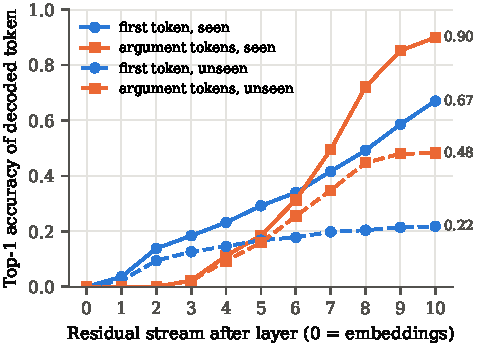
\includegraphics[width=\linewidth]{figures/logit_lens.pdf}
  \caption{Logit lens.}
  \label{fig:lens}
\end{subfigure}\hfill
\begin{subfigure}[t]{0.58\textwidth}
  \centering
  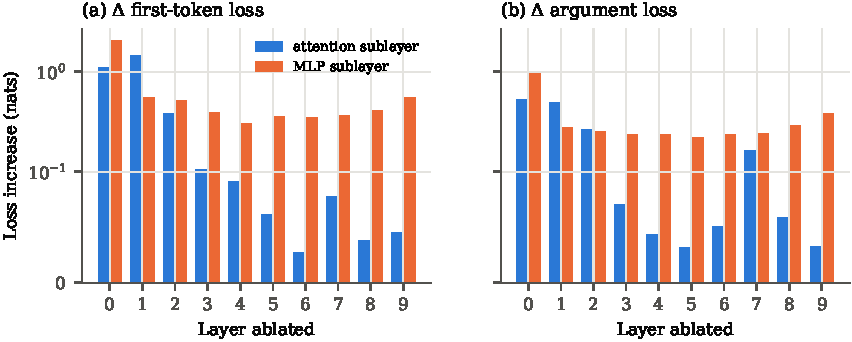
\includegraphics[width=\linewidth]{figures/sublayer_ablation.pdf}
  \caption{Zero-ablating one sublayer (seen pages).}
  \label{fig:sublayer}
\end{subfigure}
\caption{\textbf{(a)} Top-1 accuracy of decoding the residual stream after
each layer with the final norm and unembedding. Argument tokens become
decodable late (layers 7--10); on unseen pages the family token plateaus at
$\approx 0.2$ from layer 6 on. \textbf{(b)} Loss increase from removing an
entire attention or MLP sublayer (symlog scale). Attention matters in layers
0--2 and little thereafter; every MLP matters.}
\label{fig:where}
\end{figure}

\textbf{Read early, look up everywhere.} Removing the attention sublayer of
layers 0, 1, or 2 raises first-token loss by $+1.10$, $+1.44$, and $+0.38$
nats; for layers 3--9 the increase is at most $+0.10$
(\cref{fig:sublayer}). MLP sublayers are uniformly important (between $+0.31$
and $+0.56$ nats each), with layer 0's MLP the single most critical
component ($+2.04$ first-token, $+1.00$ argument loss), consistent with an
early MLP that enriches token embeddings. In this model, then, attention
mostly moves request information into the generating position in the first
three layers, and MLPs at every depth transform it---the key--value memory
picture of \citet{geva2021kv}.

\textbf{Arguments resolve late; unseen families never resolve.} The logit
lens \citep{nostalgebraist2020logitlens} (\cref{fig:lens}) shows argument
tokens on seen pages becoming decodable only from layer 7 on
($0.49\!\to\!0.90$ top-1 accuracy over layers 7--10), while the family token
rises gradually ($0.14$ after layer 2, $0.67$ at the output). On unseen pages
the family token stalls at $0.17$--$0.22$ from layer 5 onward: the later
layers that sharpen seen-page predictions have no stored association to
retrieve. Argument accuracy on unseen pages still reaches $0.48$, matching the
behavioural finding that the model copies entities from the request even when
it picks the wrong tool.

\begin{figure}[t]
\centering
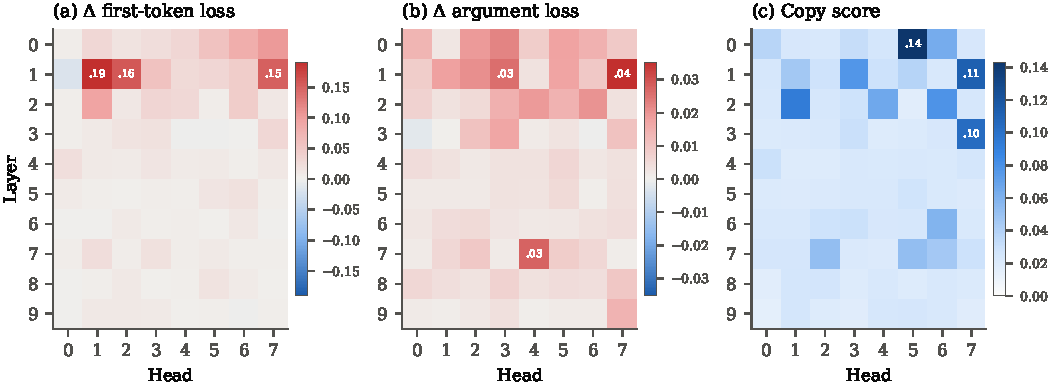
\includegraphics[width=\textwidth]{figures/head_maps.pdf}
\caption{Per-head analysis on seen pages. \textbf{(a, b)} Loss change when a
single head is zero-ablated. \textbf{(c)} Copy score: mean attention mass from
a generating position to prompt tokens identical to the token being
generated. The heads that matter, and the copying heads, are concentrated in
layers 0--3.}
\label{fig:heads}
\end{figure}

\textbf{Copy heads.} Single-head ablations (\cref{fig:heads}) are small
individually (largest: L1H1 $+0.19$ first-token loss; L1H7 $+0.035$
argument loss), indicating redundancy. The copy score isolates a handful of
early heads---L0H5 ($0.14$), L1H7 ($0.11$), L3H7 ($0.10$), L2H1 ($0.09$)---that
attend from the generating position to the matching prompt token, the
copying behaviour described by \citet{olsson2022induction}. L1H7 is both a top
copy head and the head whose removal most hurts argument loss.

\subsection{How much can be removed}
\label{sec:inside-prune}

\begin{figure}[t]
\centering
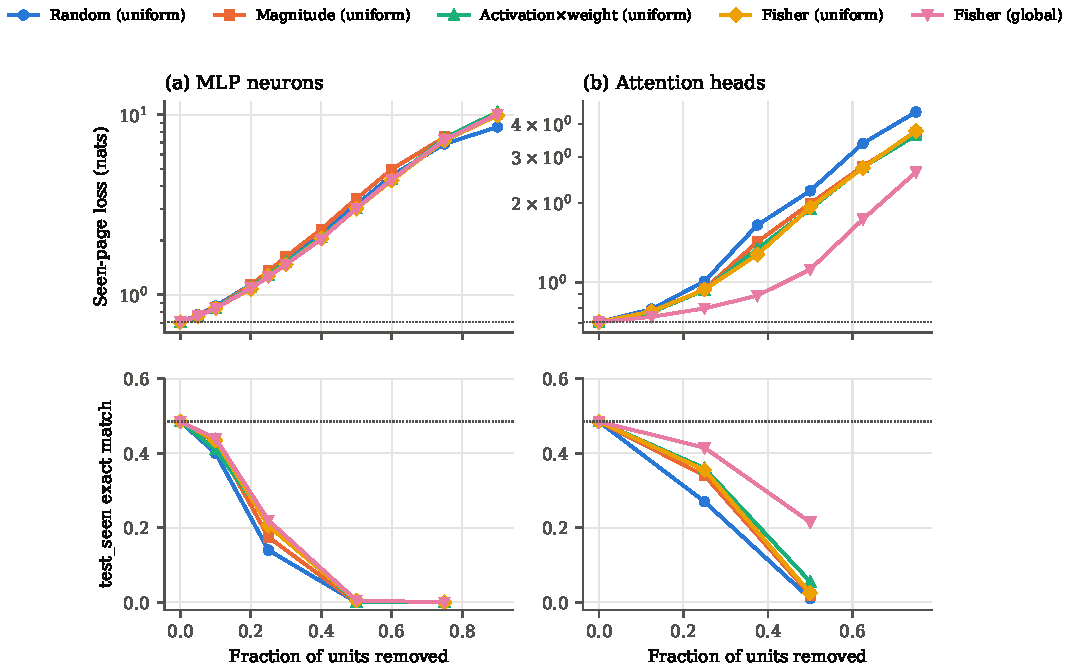
\includegraphics[width=\textwidth]{figures/pruning_curves.pdf}
\caption{Post-training pruning without recovery. Top: seen-page loss (log
scale); bottom: \texttt{test\_seen} exact match ($n{=}200$). Dotted lines are
the dense model. For MLP neurons \textbf{(a)}, no scoring rule meaningfully
beats random; for attention heads \textbf{(b)}, the Fisher score with global
allocation is far better than every alternative.}
\label{fig:curves}
\end{figure}

\begin{table}[t]
\centering\small
\setlength{\tabcolsep}{4pt}
\begin{tabular}{llcccccc}
\toprule
 & & \multicolumn{2}{c}{Seen loss} & \multicolumn{2}{c}{Unseen loss} & \multicolumn{2}{c}{\texttt{test\_seen} exact} \\
\cmidrule(lr){3-4}\cmidrule(lr){5-6}\cmidrule(lr){7-8}
Units & Rule & 25\% & 50\% & 25\% & 50\% & 25\% & 50\% \\
\midrule
\multirow{5}{*}{\shortstack[l]{MLP\\neurons}}
 & random & 1.342 & 3.155 & 4.128 & 4.833 & 0.140 & 0.000 \\
 & magnitude & 1.351 & 3.415 & 4.120 & 4.944 & 0.175 & 0.000 \\
 & activation$\times$weight & 1.283 & 3.004 & 4.131 & \best{4.691} & 0.215 & 0.000 \\
 & Fisher (uniform) & 1.274 & \best{3.002} & 4.138 & 4.736 & 0.205 & 0.005 \\
 & Fisher (global) & \best{1.257} & 3.022 & \best{4.112} & 4.764 & \best{0.220} & 0.005 \\
\midrule
\multirow{5}{*}{\shortstack[l]{Attention\\heads}}
 & random & 1.008 & 2.226 & 4.291 & 4.717 & 0.270 & 0.010 \\
 & magnitude & 0.941 & 1.992 & 4.247 & 4.566 & 0.340 & 0.020 \\
 & activation$\times$weight & 0.933 & 1.901 & 4.252 & 4.537 & 0.360 & 0.055 \\
 & Fisher (uniform) & 0.937 & 1.926 & 4.268 & 4.605 & 0.355 & 0.025 \\
 & Fisher (global) & \best{0.795} & \best{1.119} & \best{4.200} & \best{4.402} & \best{0.415} & \best{0.215} \\
\bottomrule
\end{tabular}
\caption{Fraction of units removed vs.\ quality, no recovery. Dense model:
seen loss $0.705$, unseen loss $4.146$, \texttt{test\_seen} exact $0.485$ on
this 200-request subset (Wilson interval $\pm 0.07$).}
\label{tab:prune}
\end{table}

\textbf{There are no free MLP neurons.} Every scoring rule tracks random
pruning closely (\cref{fig:curves}a, \cref{tab:prune}): at 50\% of MLP
neurons removed, seen loss is $3.00$--$3.42$ nats for all rules against
$3.16$ for random, and generation collapses to $\leq 0.005$ exact for all.
Even 10\% removal costs 5--9 exact points (dense $0.485$ $\to$
$0.400$--$0.440$). The scores barely agree with each other: the bottom halves
selected by Fisher and by random overlap at $0.507$ (chance is $0.5$), and
only magnitude and activation, which share a weight-norm factor, overlap
substantially ($0.84$). Fisher-global, free to choose per-layer budgets,
spreads pruning almost uniformly (per-layer sparsity $0.45$--$0.53$ at a 50\%
target). This is the opposite of the large-model regime, where 20--50\% of
structure can often be removed with little loss
\citep{ma2023llmpruner,ashkboos2024slicegpt,men2024shortgpt}: a 9.6M model
trained on 100M tokens of its task has no spare MLP capacity, and every
neuron carries a small share of the stored command knowledge.

\textbf{Heads are prunable---if allocation is global.} For attention heads,
Fisher-global is in a different class (\cref{fig:curves}b): removing 25\% of
heads (20 of 80; 0.66M parameters) costs $0.09$ nats and 7 exact points,
against 22 points for random; at 50\%, it retains $0.215$ exact where random
retains $0.010$. Its allocation is the mechanism: it removes \emph{no} head
from layers 0--2 and 62--88\% of heads from layers 3--6 and 8--9 at the 50\%
target, mirroring the sublayer ablations. Uniform allocation, even with the
same Fisher scores, is no better than magnitude, because it is forced to
remove the critical early heads.

\textbf{Pruning helps unseen-page loss slightly, and it is not knowledge.}
Removing up to 25\% of MLP neurons, by any rule, leaves unseen-page loss flat
or slightly \emph{lower} ($4.146\!\to\!4.09$--$4.14$) while seen-page loss
nearly doubles. Unseen first-token loss falls from $5.90$ to $5.67$ under
Fisher pruning at 30\%. Generation on unseen pages, however, does not improve
(command match $0.150\!\to\!0.135$--$0.160$ at 10\%). We read this as a calibration effect:
on unseen pages the dense model is confidently wrong, and damaging the
network softens its predictions, which lowers cross-entropy without making
them more correct.

\subsection{Is page memory localized?}
\label{sec:inside-diff}

\begin{figure}[t]
\centering
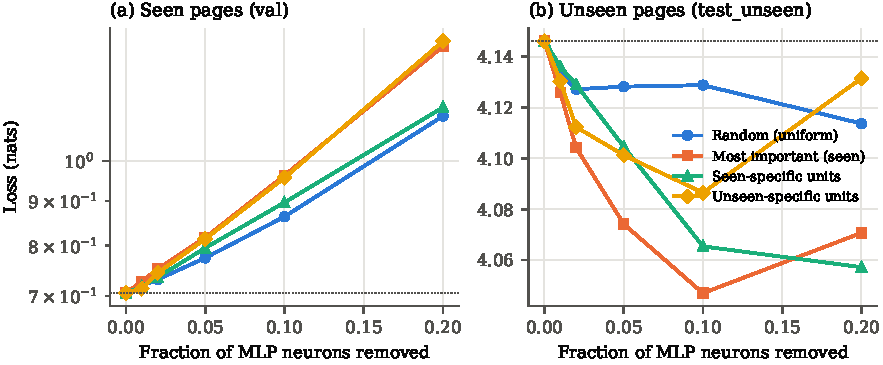
\includegraphics[width=\textwidth]{figures/differential.pdf}
\caption{Differential pruning of MLP neurons. ``Seen-specific'' removes the
units with the largest gap between normalized Fisher importance on seen and
unseen pages; ``most important (seen)'' removes the top Fisher units.}
\label{fig:diff}
\end{figure}

If the knowledge of seen pages lived in a small set of ``page neurons''
\citep{dai2022knowledge,meng2022rome}, removing the units most important on
seen pages but unimportant on unseen pages should hurt seen pages sharply and
spare unseen pages. We rank units by the difference of their normalized
Fisher scores on training requests and on \texttt{val\_unseen} (scores and
evaluation sets are disjoint) and compare against removing the most
important seen-page units, the most \emph{unseen}-specific units, and random
units (\cref{fig:diff}).

The prediction fails. At 20\% removal, seen-specific pruning yields seen loss
$1.153$ against $1.126$ for random; even removing the 20\% of units with the
\emph{highest} seen-page Fisher score yields only $1.354$, a $+0.23$-nat gap
over random. Unseen loss stays within $0.10$ nats of the dense model under all
four rules, and at 10\% the seen-specific model generates no better than random on unseen
pages (command match $0.150$ vs.\ $0.160$). Seen and unseen Fisher rankings
correlate only weakly (Spearman $0.33$). Within the resolution of this
experiment, page knowledge in \modelname{} is \emph{distributed}: importance is
spread thinly over most MLP units, matching recent doubts that memorization
localizes to few units \citep{chang2024localization} and the observation that
compression erodes long-tail knowledge first and broadly
\citep{hooker2019forget}.

\subsection{Recovery and real savings}
\label{sec:inside-recovery}

Pruning without recovery is a probe, not a compression method. We therefore
fine-tune pruned models with their masks fixed for 400 steps (batch 32, i.e.\
12{,}800 training requests, about 1\% of one epoch; AdamW, lr $10^{-4}$) on
$\tfrac12$ cross-entropy plus $\tfrac12$ KL divergence to the dense model's
token distribution \citep{hinton2015distilling,muralidharan2024minitron}, then
\emph{physically} slice the MLP matrices and time single-request decoding with
the reference decoder (\cref{tab:recovery}).

\begin{table}[t]
\centering\footnotesize
\setlength{\tabcolsep}{3.5pt}
\begin{tabular}{lrcccccc}
\toprule
MLP neurons removed & Params & Seen loss & Unseen loss & Exact & Command & Token F1 & p50 \\
\midrule
none (dense) & 9.57M & 0.705 & 4.146 & 0.485 & 0.675 & 0.625 & 238\,ms \\
\midrule
50\%, Fisher-global, no recovery & 6.62M & 3.022 & 4.764 & 0.005 & 0.125 & 0.071 & -- \\
50\%, Fisher-global + 400 steps & 6.62M & \best{1.565} & 3.877 & \best{0.160} & 0.375 & \best{0.408} & 248\,ms \\
50\%, random + 400 steps & 6.62M & 1.636 & 3.898 & 0.150 & \best{0.390} & 0.374 & 238\,ms \\
\midrule
75\%, Fisher-global, no recovery & 5.15M & 7.256 & 7.696 & 0.000 & 0.010 & 0.020 & -- \\
75\%, Fisher-global + 400 steps & 5.15M & 2.227 & \best{3.759} & 0.025 & 0.265 & 0.275 & 199\,ms \\
\bottomrule
\end{tabular}
\caption{Masked distillation after MLP pruning. Generation metrics on 200
\texttt{test\_seen} requests. Parameters are those of the physically sliced
model (max logit difference to the masked model $\leq 4\cdot 10^{-6}$).}
\label{tab:recovery}
\end{table}

Three observations. First, recovery is real but partial at this budget: 50\%
pruning plus 400 steps returns from $0.005$ to $0.160$ exact (dense
$0.485$). Second, after recovery the scoring rule hardly matters (Fisher
$0.160$ vs.\ random $0.150$, within noise at $n{=}200$), as one would expect if
no subset of neurons is special. Third, \emph{parameters are not latency}:
the 6.62M sliced model decodes no faster than the dense one ($248$ vs.\
$238$\,ms p50) and the 5.15M model only 16\% faster. At batch size 1 on a CPU,
per-token cost is dominated by attention over the growing context, the
$4{,}096\times256$ unembedding, and framework overhead, not by MLP
arithmetic. Recovered models again show \emph{lower} unseen-page loss than
the dense model ($3.76$--$3.90$ vs.\ $4.15$) with no gain in unseen-page
generation, reinforcing the calibration reading of \cref{sec:inside-prune}.

\subsection{Extracting a specialist}
\label{sec:inside-family}

The negative results above concern a model asked to keep \emph{all} of its
3{,}651 command families. A practical alternative is to keep only the
families a given user needs. We score units by Fisher importance on 512
training requests from ten DevOps families (\texttt{git}, \texttt{docker},
\texttt{kubectl}, \texttt{systemctl}, \texttt{cargo}, \texttt{npm},
\texttt{pip}, \texttt{terraform}, \texttt{aws}, \texttt{helm}), remove MLP
neurons and heads by global ranking, distill for 400 steps on the same family
data, and evaluate on 200 held-out family requests (seen pages, held-out
styles: \texttt{val}, \texttt{test\_seen}, \texttt{test\_paraphrase}) and on
183 \texttt{test\_seen} requests from all other families
(\cref{tab:family}).

\begin{table}[t]
\centering\footnotesize
\setlength{\tabcolsep}{4pt}
\begin{tabular}{lrcccc}
\toprule
 & & \multicolumn{3}{c}{Ten target families ($n{=}200$)} & Other ($n{=}183$) \\
\cmidrule(lr){3-5}\cmidrule(lr){6-6}
Model & Params & Exact & Command & Token F1 & Exact \\
\midrule
Dense generalist & 9.57M & \best{0.465} & 0.790 & \best{0.625} & \best{0.470} \\
50\% MLP, family scores, no recovery & 6.62M & 0.010 & 0.615 & 0.120 & 0.011 \\
50\% MLP, general scores, no recovery & 6.62M & 0.000 & 0.465 & 0.075 & 0.005 \\
\midrule
Specialist: 75\% MLP, 25\% heads + 400 steps & 4.49M & 0.395 & 0.895 & 0.605 & 0.000 \\
Specialist: 90\% MLP, 50\% heads + 400 steps & 2.95M & 0.300 & \best{0.910} & 0.535 & 0.000 \\
\bottomrule
\end{tabular}
\caption{Extracting a ten-family specialist from the 9.6M generalist.
Parameters count the sliced MLPs and treat masked heads as removed. Without
recovery, no mask preserves the target families; with 400 steps of
family-data distillation, a 2.95M subnetwork keeps 65\% of the dense
model's exact match on its families and selects the family more often than
the dense model. Wilson half-widths are about $\pm0.07$.}
\label{tab:family}
\end{table}

Before recovery, family-specific scores protect the target families slightly
better than general scores (command match $0.615$ vs.\ $0.465$ at 50\%), but
no mask preserves exact match. After recovery, the specialists behave very
differently from generally pruned models: the 4.49M specialist reaches $0.395$
exact on its families ($85\%$ of the dense model's $0.465$) and the 2.95M
specialist $0.300$ ($65\%$), while both choose the right family \emph{more}
often than the dense model ($0.895$ and $0.910$ vs.\ $0.790$), because they no
longer compete with thousands of other command families---the label-space effect of
\cref{sec:core} reappearing. Everything else is forgotten (exact $0.000$ on
other families). By contrast, the 2.1M core model of \cref{sec:core}, trained
from scratch on $\sim$100 families, reached only $0.028$--$0.057$ exact; the
family sets and evaluation sets differ, so we read the comparison as
directional evidence that \emph{carving a specialist out of a larger
generalist} beats training a specialist of similar size from scratch on this
budget.

\begin{finding}{RQ5}
Early attention (layers 0--2) reads the request and a few early heads copy its
entities; MLPs at every depth hold command knowledge, and unseen-page
predictions stall mid-network for lack of anything to retrieve. In this
small-relative-to-data regime, MLP neurons are uniformly necessary (no scoring
rule beats random; 10\% removal costs 5--9 exact points) while attention heads
are prunable when allocation is global (25\% of heads for 7 points). Page
knowledge is distributed rather than localized. Compression that keeps
\emph{everything} is therefore expensive here, but compression that keeps a
\emph{chosen subset} of families works: a distilled 2.95M subnetwork keeps
65\% of the generalist's exact match on ten families.
\end{finding}
